\chapter{Limbajul de programare Java}

\section{Platforma Java}
\vspace{1cm}
\begin{defn}
Java este un limbaj de programare orientat-obiect, puternic tipizat, conceput de către James Gosling la Sun Microsystems (acum filială Oracle) la începutul anilor '90, fiind lansat în 1995. Cele mai multe aplicații distribuite sunt scrise în Java, iar noile evoluții tehnologice permit utilizarea sa și pe dispozitive mobile gen telefon, agenda electronică, palmtop etc. În felul acesta se creează o platformă unică, la nivelul programatorului, deasupra unui mediu eterogen extrem de diversificat. Acesta este utilizat în prezent cu succes și pentru programarea aplicațiilor destinate intranet-urilor. \cite{12}
\end{defn}
Java este un limbaj de programare utilizat în toate industriile pentru aproape orice tip de aplicație. Există aproximativ 6 milioane de programatori Java în lume, însă sunt de asemenea și multe posturi disponibile, astfel că un programator care are cunoștințe medii de programare Java are mai multe șanse să-si gasească un job față de un programator expert în alte limbare de programare precum C/C++, Ruby, etc.
\paragraph{ }Java a apărut pe scena tehnologiei în anul 1995 și a devenit popular foarte repede. Acest lucru s-a întâmplat în parte din cauza JVM.
JVM este ca un translator de limbi străine, având loc transformarea bytecode-ului Java în orice limbaj nativ ce poate fi interpretat de un anumit calculator.\cite{10}\newline
Programele Java sunt rulate (sau interpretate) de către un alt program numit Java VM. Programele nu rulează direct pe sistemul de operare nativ, ci sunt interpretate de Java VM pentru sistemul de operare nativ.\newpage Acest lucru înseamnă că orice sistem de operare cu Java VM instalat poate rula programe Java, indiferent de sistemul de operare pe care au fost dezvoltate inițial aplicațiile.\newline
 Aceasta se numește portabilitate, și în lumea programării, portabilitatea este un produs foarte prețios.\cite{11} \newline

Platforma Java constă în API-ul Java și mașina virtuală Java (JVM).

\paragraph{ }API-urile Java sunt biblioteci de cod compilat care se folosesc în dezvoltarea programelor java. Acestea permit adăugarea unor funcționalității personalizabile pentru a economisi timp de programare, unul dintre cele mai simple exemple fiind reprezentat de API-ul folosit pentru a printa o linie de cod în consolă; comanda pentru printare în consolă este furnizată din API și poate fi folosită numai prin specificarea textului ce va fi printat. \newline

De exemplu, un program Java dezvoltat pe un computer personal (PC) cu sistemul de operare Windows NT ar trebui să ruleze la fel de bine fără modificări pe o stație de lucru cu sistem de operare Linux, și vice-versa.\cite{10}\newline 

\section{Configurarea unui computer}

Pentru a scrie programe Java, sunt necesare:
\begin{itemize}
  \item un compilator Java
	\item un JVM
	\item API-ul Java
	\item acces la documentația API-ului Java
	\item un editor pentru redactarea programelor Java.
	\item un program care să interpreteze și să execute comenzile redactate 
\end{itemize}
Pentru ultimele două acțiuni se folosește, în general, o singură interfață prietenoasă, numită mediu de dezvoltare integrat(integrated development environment - IDE).
Printre cele mai cunoscute IDE - uri utilizate pentru dezvoltarea de aplicații Java se numără: Eclipse, NetBeans, IntelliJ IDEA, JDeveloper, JCreator, etc.\newpage

În procesul de realizare a aplicației mele, am utilizat pentru programul de citire a link-urilor și actualizarea periodică a bazei de date,  ca și mediu de dezvoltare integrat Eclipse IDE, deoarece:\newline
\begin{itemize}
	\item poate fi descărcat și apoi utilizat gratuit
	\item este în topul celor mai utilizate Java IDE-uri de către programatorii consacrați
	\item este intuitiv și ușor de utilizat
\end{itemize}
\paragraph{ }Eclipse nu este folosit doar pentru dezvoltarea unei aplicații Java, ci poate fi folosit împreună cu o serie de alte limbaje de programare (Ada, ABAP, C, C++, COBOL, Fortran, Haskell, JavaScript, Lasso, Lua, Natural, Perl, PHP, Prolog, Python, R, Ruby, Scala, Clojure, Groovy, Scheme și Erlang), acest lucru reprezentând un plus semnificativ al acestui IDE.\newline



\textbf{JDK și JRE}\newline
Pentru dezvoltarea de programe Java pe un computer este nevoie să fie instalat JDK. Pentru rularea de programe Java care au fost compilate deja pe un alt computer, este de ajuns Java Runtime Environment (JRE). 
JDK include si JRE.

\section{Limbaj de programare obiect orientat}

Java este un limbaj de programare obiect orientat, ceea ce înseamnă că se pot construi si reprezenta obiecte din lumea reală. Fiecare program Java are cel putin o clasă care are anumite funcționalități. De exemplu, cea mai simplă clasă, HelloWorld, are funcționalitatea de a saluta lumea.
Clasele în Java pot să conțină metode(funcții) și atribute (proprietăți).\newline
\textbf{Principiile programării obiect orientate }\newline
\subsection{Abstractizarea datelor}
Abstractizarea datelor reprezintă procesul de definire a unui tip de date denumit tip abstract de date(abstract data type-ADT), recurgând și la ascunderea datelor.
Definirea unui tip abstract de date implică specificarea reprezentării interne a datelor pentru acel tip, precum și un set suficient de funcții cu ajutorul cărora putem utiliza acel tip fără a fi necesară cunoașterea structurii sale interne. \cite{15}

\subsection{Încapsularea}
Încapsularea se referă la ascunderea datelor și a metodelor într-un obiect., prin specificarea acestora ca fiind private în definiția clasei. Astfel, accesul la date se face doar prin intermediul metodelor descrise în clasă. Încapsularea este importantă pentru a asigura securitatea și integritatea obiectelor unei clase.  
Un mare avantaj al încapsulării este ascunderea implementării clasei astfel că metodele interne ale clasei pot fi modificate după cum vrea programatorul și atâta timp cât funcționalitatea externă nu este modificată, utilizatorul clasei nu va observa nicio diferență la utilizarea metodei.\cite{14}

\subsection{Moștenirea}
În limbajele de programare obiect-orientate, termenul de moștenire se referă la abilitatea de a defini o nouă clasă bazată pe una care deja există.
Clasa utilizată ca și clasă de bază poate fi definită de aceeași persoană, poate fi preluată de la altcineva sau dintr-un pachet Java specific.
Clasa derivată din clasa de bază se mai numește subclasă, clasă copil iar cea de bază se mai numește și superclasă, clasă părinte. 
Clasa derivată va moșteni de la superclasa sa toate funcționalitățile pe care aceasta le are dar poate să conțină și funcționalități noi sau să le suprascrie pe cele existente.\cite{14}

În figura următoare se observă o ierarhie de clase realizată prin moștenire:
\begin{figure}[!hp]
\centering
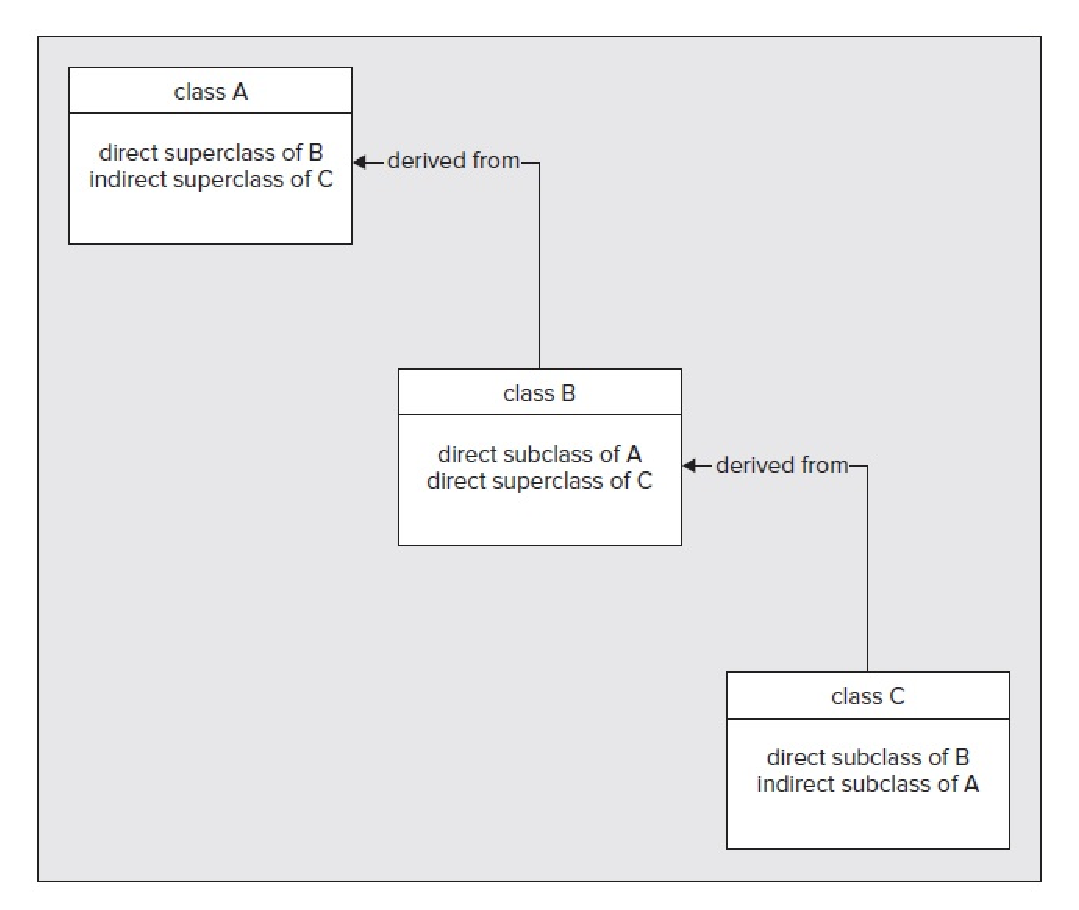
\includegraphics[width=0.9\textwidth]
{imagini/mostenire1.eps}
\end{figure}

După cum puteți vedea în Figura , o subclasă care se află în același pachet ca și clasa de bază moștenește totul cu excepția membrilor privați ai clasei de bază. Dacă se definește o subclasă în afara pachetului ce conține clasa de bază, atributele private nu sunt mostenite și nici ceilalți membrii din clasa de bază care au fost declarați fără specificator de acces sau cei declarați ca private.\newline
\begin{figure}[!hp]
\centering
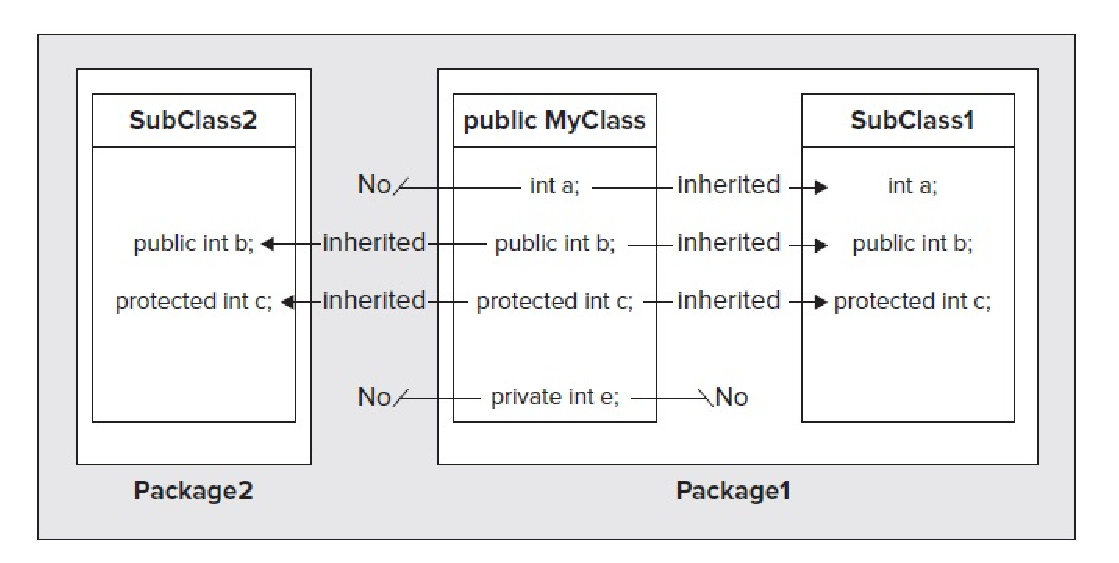
\includegraphics[width=0.9\textwidth]
{imagini/mostenire2.eps}
\end{figure}
Astfel, specificatorul public este cel mai puțin restrictiv, fiind vizibil oriunde, protected este următorul care previne accesul din clasele aflate în afara pachetului dar nu limitează moștenirea, clasa derivată poate să accese membrii clasei de bază declarați protected. Cel mai restrictiv specificator este private, accesul fiind valabil doar în interiorul clasei în care a fost declarat mebrul privat.

\subsection{Suprascrierea unei metode}
Un alt termen important din programarea obiect-orientată este reprezentat de către suprascrierea metodelor.
Putem defini o metodă într-o clasă derivată, care are aceeași semnătură ca și o metodă în clasa de bază. Având aceeași semnătură înseamnă că numele metodei trebuie să fie același și listele de parametri trebuie să conțină același număr de parametri cu tipuri identice. Atributul de acces pentru metoda în clasa derivată poate fi același cu cel din clasa de bază sau poate fi mai puțin restrictiv, dar nu poate fi mai restrictiv. Acest lucru înseamnă că, dacă declaram o metodă publică în clasa de baza, orice proprietate definită în clasa derivată trebuie să fie, de asemenea, declarată ca publică. Nu se poate omite atributul de acces în clasa derivată în acest caz, sau specificarea aceastuia ca fiind private sau protected.
Când se definește o nouă versiune a unei metode din clasa de bază în acest fel, metoda din clasă derivată suprascrie metoda din clasa de baz. \cite{14} \newline

\subsection{Adnotarea @Overriding}
Când se definește o metodă într-o clasă derivată, care este destinată pentru a suprascrie o metodă din superclasă, este ușor să se facă o greșeală în semnătura pentru metoda de clasă derivată. Dacă numele și lista de parametri din metoda clasei derivate nu sunt identice cu cele ale metodei din superclasa, are loc supraîncărcarea metodei din clasa de bază și nu suprascrierea acesteia. Pentru evitarea acestui lucru și pentru o mai bună lizibilitate a codului scris se folosește adnotarea @Overriding înainte de metoda care va suprascrie metoda din clasa de bază. Astfel compilatorul este informat și în caz că nu sunt indeplinite toate condițiile de suprascriere se va semnala o eroare de compilare.\cite{14} \newline

\subsection{Polimorfismul}
Polimosfismul înseamnă, în general, abilitatea de a avea mai multe forme. În programare, reprezintă abilitatea unei singure variabile de un tip dat să fie utilizată pentru a referi obiecte de tipuri diferite și să apeleze automat metoda specifică tipului obiectului referit. Aceasta presupune faptul că o singură metodă poate să se comporte diferit, în funcție de obiectul apelat.\newline
Acest lucru este evidențiat în figura următoare:\cite{14} 
\begin{figure}[!hp]
\centering
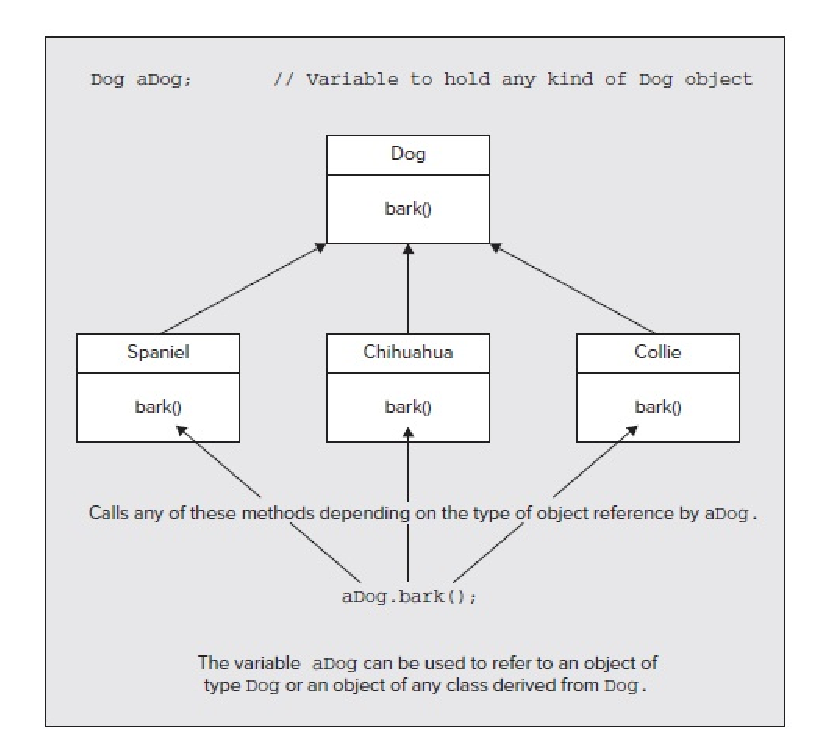
\includegraphics[width=0.9\textwidth]
{imagini/polimorfism.eps}
\end{figure}
\paragraph{}Condițiile care trebuiesc îndeplinite pentru a utiliza polimorfismul sunt următoarele:\cite{14} 
\begin{itemize}
	\item apelul metodei din clasa derivată trebuie să se facă prin intermediul unei variabile de tipul clasei de bază
	\item metoda apelată trebuie să fie definită în clasa de derivată
	\item metoda apelată trebuie să fie, de asemenea, declarată ca membru al clasei de bază
	\item semnătura metodei din clasa de bază trebuie să fie la fel cu semnătura metodei din clasa derivată sau tipurile returnate să fie covariante
	\item specificatorul de acces din clasa derivată nu trebuie să fie mai restrictiv ca specificatorul de acces din clasa de bază
\end{itemize}
\subsection{Clasa de bază universală}
Toate clasele definite în Java sunt implicit subclase ale clasei Object, nefiind nevoie să fie specificat acest lucru.
Astfel, cu ajutorul clasei Object, putem să scriem metode care vor utiliza obiecte de tipuri necunoscute, putem să definim parametri de tip Object, în acest fel metoda va putea fi folosită pentru orice tip de obiect trimis ca parametru. De asemenea, clasa Object cuprinde 7 metode publice și 2 protejate, pe care le vom vedea în tabelul următor:\cite{14} \newpage
\begin{center}
\begin{table}[!hp]
\caption{Metodele publice ale clasei Object}
\begin{tabular}{|p{4cm}|p{8cm}|}\hiderowcolors
\hline
\cellcolor{LightPink} Metodă & \cellcolor{LightGreen} Scopul metodei \\
toString()& Această metodă returnează un obiect String care descrie obiectul curent. În versiunea moștenită a acestei metode va fi returnat numele clasei urmat de ‘@’ și de reprezentarea hexazecimală a obiectului. Această metodă este apelată automat atunci când se concatenează obiecte cu variabile String utilizând operatorul +. Această metodă poate fi suprascrisă într-o clasă, pentru a crea un string personalizat pentru obiectul clasei. \\
\hline
equals() & Această metodă compară referința la obiectul trimis ca argument cu referința la obiectul curent și returnează true, dacă acestea sunt egale. True este returnat dacă obiectul curent și argumentul reprezintă același obiect, nu au doar valorile egale iar false este returnat dacă sunt obiecte diferite chiar și dacă atributele acestora au valori identice.\\
\hline
getClass()& Această metodă returnează un obiect de tipul Class care identifică clasa obiectului curent.\\
\hline
hashCode()& Această metodă calculează valoarea hashcode pentru un obiect și o returnează ca int. Valorile hashcode sunt utilizate in clasele definite în pachetul java.util pentru a memora obiectele în tabele de dispersie (tabele hash).\\
\hline
notify()& Această metodă este folosită pentru a "`trezi"' un fir de execuție asociat cu obiectul curent.\\
\hline
notifyAll()& Această metodă este folosită pentru a "`trezi"' toate firele de execuție asociat cu obiectul curent.\\
\hline
wait()& Această metodă este folosită pentru a determina un fir de execuție să aștepte o schimbare în obiectul curent.\\
\hline
\end{tabular}
\end{table}
\end{center}
De reținut că metodele  getClass(), notify(), notifyAll() și wait() nu pot fi suprascrise într-o clasă definită de noi întrucât sunt specificate ca fiind finale în definiția clasei Object.\newpage
Pentru metoda toString() este sugerat să utilizăm mereu adnotarea @Override în clasa noastră pentru a nu se folosi polimorfismul prin apelarea metodei din clasa Object.\newline

Cele două metode protected ale clasei Object sunt:\newline
\begin{center}
\begin{table}[!hp]
\caption{Metodele protejate ale clasei Object}
\begin{tabular}{|p{4cm}|p{8cm}|}\hiderowcolors
\hline
\cellcolor{LightPink} Metodă & \cellcolor{LightGreen} Scopul metodei \\
clone()& Această metodă creează un obiect care este o copie a obiectului curent fără să țină cont de tipul acestuia, poate fi de orice tip. Acest lucru poate fi realizat doar dacă  obiectul ce urmează a fi clonat indică faptul că este acceptată clonarea sa prin implementarea interfeței Cloneable.\\
\hline
finalize() & Această metodă poate fi apelată pentru a ,,curăța'' după ce un obiect a fost distrus.\\
\hline
\end{tabular}
\end{table}
\end{center}
Utilizarea metodei clone() pentru a duplica obiectele poate fi complicată și dacă nu se realizează corect poate să ducă la rezultate neașteptate. De aceea pentru a clona obiecte ale clasei definite de noi este indicat să utilizăm un constructor de copiere. 







